% requires \usepackage{subcaption}
\begin{figure}[H]
    \centering
    \begin{subfigure}{0.34\textwidth}
        \centering
        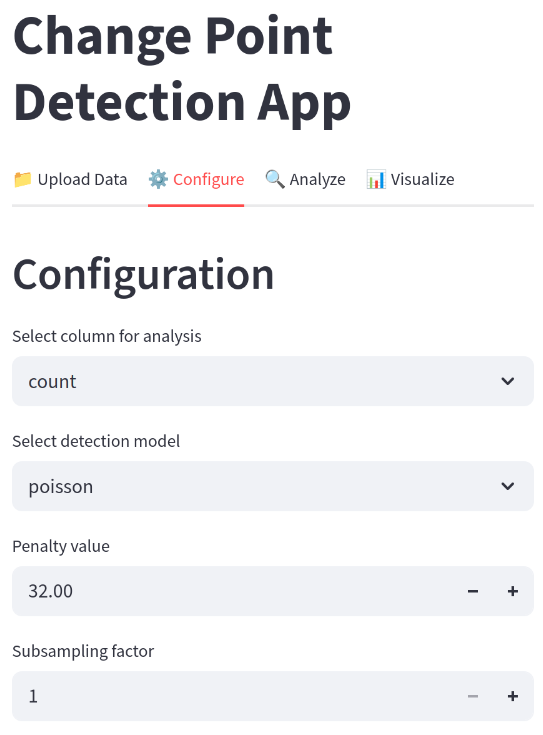
\includegraphics[width=\textwidth]{figures/changepoints-settings.png}
        \caption{Web app: settings}
        \label{fig:changepoints-settings}
    \end{subfigure}
    \hfill
    \begin{subfigure}{0.65\textwidth}
        \centering
        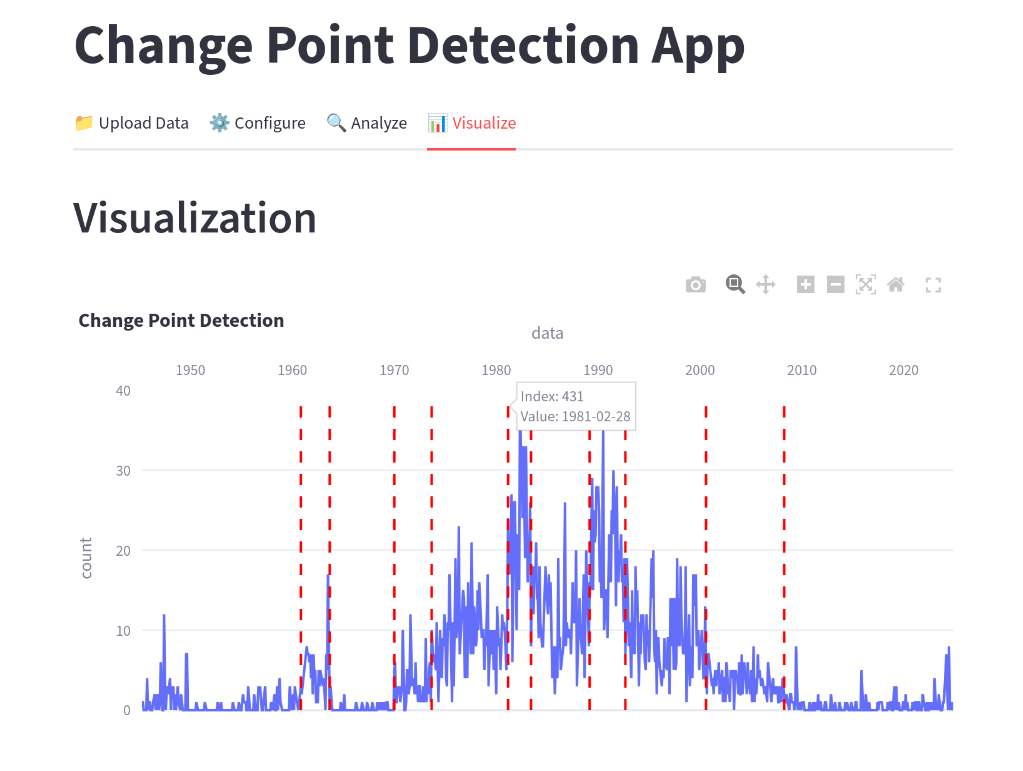
\includegraphics[width=\textwidth]{figures/changepoints.png}
        \caption{Web app: changepoint view}
        \label{fig:changepoints-webapp}
    \end{subfigure}
    \caption{
        Screenshots of the web application developed to visualize and explore the changepoint detection results. From the settings panel (\subref{fig:changepoints-settings}) it's possible to configure the algorithm parameters; the main view (\subref{fig:changepoints-webapp}) shows the time series of murders with detected changepoints in red dashed lines.
    }
    \label{fig:changepoints-webapp-full}
\end{figure}